%%%%%%%%%%%%%%%%%%%%%%%%%%%%%%%%%%%%%%%%%%%%%%%%%%%%%%%%%%%%%%%%%%%%
% PREAMBLE
%%%%%%%%%%%%%%%%%%%%%%%%%%%%%%%%%%%%%%%%%%%%%%%%%%%%%%%%%%%%%%%%%%%%

\documentclass[handout]{beamer}
%\documentclass{beamer}

%------------------------------------------------------------------
% Presentation Settings
%------------------------------------------------------------------

\mode<presentation>
{
	\usetheme{Boadilla}      % or Boadilla, Singapore, ...
	\usecolortheme{default} % or albatross, beaver, crane, ...
	\usefonttheme{default}  % or serif, structurebold, ...
	\setbeamertemplate{navigation symbols}{}
	\setbeamertemplate{caption}[numbered]
	\setbeamertemplate{itemize items}[circle]
	\setbeamertemplate{itemize subitem}[triangle]
	\setbeamertemplate{enumerate items}[default]
	\setbeamerfont{caption}{size=\tiny}
	%\setbeamercolor{alerted text}{fg=blue}
}

%------------------------------------------------------------------
% Packages
%------------------------------------------------------------------
\usepackage{amsmath}
\usepackage[natbibapa]{apacite}
\usepackage{appendixnumberbeamer}
\usepackage[english]{babel}
\usepackage{comment}
\usepackage{hyperref}
\usepackage[utf8x]{inputenc}
\usepackage{pdfpages}
\usepackage{subcaption}
\usepackage{verbatim}

\usepackage{listings} % Code blocks
\usepackage{color}

\definecolor{ltgreen}{RGB}{230, 242, 230}

\lstset{frame=tb,
  language=bash,
  aboveskip=3mm,
  belowskip=3mm,
  showstringspaces=false,
  columns=flexible,
  basicstyle={\small\ttfamily},
  numbers=none,
  breaklines=true,
  breakatwhitespace=true,
  tabsize=3,
  backgroundcolor=\color{ltgreen}
}


%------------------------------------------------------------------
% Set up
%------------------------------------------------------------------

% Add section titles

\AtBeginSection[]{
	\begin{frame}
  	\vfill
  	\centering
  	\begin{beamercolorbox}[sep=8pt,center,shadow=false,rounded=false]{title}
    	\usebeamerfont{title}\insertsectionhead\par%
  	\end{beamercolorbox}
  	\vfill
  \end{frame}
}

% Reduce references font size

\renewcommand*{\bibfont}{\scriptsize}

%------------------------------------------------------------------
% Title page settings
%------------------------------------------------------------------

\title[Git/GitHub Workshop: Part 4]{Workshop: Introduction to Git and GitHub}

\subtitle{Part 4: GitHub}

\author[P. Joly]{Philippe Joly}
\institute[FU-Berlin]{Freie Universität Berlin}

\date{March 9, 2021}

%%%%%%%%%%%%%%%%%%%%%%%%%%%%%%%%%%%%%%%%%%%%%%%%%%%%%%%%%%%%%%%%%%%%
% DOCUMENT
%%%%%%%%%%%%%%%%%%%%%%%%%%%%%%%%%%%%%%%%%%%%%%%%%%%%%%%%%%%%%%%%%%%%

\begin{document}

%------------------------------------------------------------------
% Title Page
%------------------------------------------------------------------
\begin{frame}
\titlepage
\end{frame}
%

%\begin{columns}
%  \begin{column}{0.5\textwidth}
%
%    ...
%
%  \end{column}
%  \begin{column}{0.5\textwidth}
%    ...
%  \end{column}
%\end{columns}

%\begin{lstlisting}
%$ cd /home/user/my_project
%\end{lstlisting}

%\begin{figure}
%	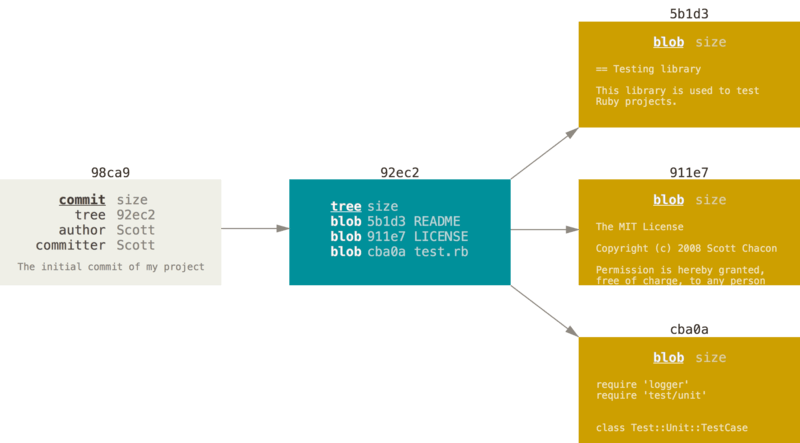
\includegraphics[width=0.9\textwidth]{figures/fig09_commit.png}
%	\caption{A commit and its tree. \textit{Source}: Chacon \& Straub (2021), fig. 9.}
%\end{figure}

%%------------------------------------------------------------------

\begin{frame}{Reference}
	\begin{columns}
	
		\begin{column}{0.5\textwidth}
			\begin{itemize}
				\item This workshop draws extensively on Scott Chacon and Ben Straub (2021), \href{https://git-scm.com/book/en/v2}{\textit{ProGit}}, Version 2.1.295, 2021-02-26. 
				\item Like the book, this workshop carries the CC BY-NC-SA 3.0 license.
			\end{itemize}
		\end{column}
		
		\begin{column}{0.5\textwidth}
			\begin{figure}
				
\includegraphics[width=0.5\textwidth]{figures/progit_cover.png}
				\caption{}
			\end{figure}
		\end{column}
	
	\end{columns}
\end{frame}

%%------------------------------------------------------------------

\section{GitHub tour}

\section{Exercise 1: A pull request inside a repo}

\begin{frame}[fragile]{Exercise 1 (a)}
1. Log into GitHub and clone the following repository (you have to be a collaborator):

\vspace{0.3cm}

(SSH)
\begin{lstlisting}
$ git clone git@github.com:jolyphil/demorepo
\end{lstlisting}

(or HTTPS)
\begin{lstlisting}
$ git clone https://github.com/jolyphil/demorepo
\end{lstlisting}

2. Open the repository on your computer.

\vspace{0.3cm}

3. Create and switch to a new branch named with your initials. 

\begin{lstlisting}
$ git checkout -b pj
\end{lstlisting}

\end{frame}


\begin{frame}[fragile]{Exercise 1 (b)}

4. Create a new script (R or Stata) that loads \texttt{data/auto.dta} and generates a PNG graph from it (e.g., \texttt{scritps/pj.do}). 

\vspace{0.3cm}

5. With this script, export a PNG graph to the \texttt{figures} folder (e.g., \texttt{figures/pj.png}).

\vspace{0.3cm}

6. Modify \texttt{paper/results.md} so that your graph will appear under your initials. 

\vspace{0.3cm}

6. Stage your changes.

\begin{lstlisting}
$ git add scripts/pj.do 
$ git add figures/pj.png
$ git add paper/results.md
\end{lstlisting}

7. Commit your changes.

\begin{lstlisting}
$ git commit -m "Add a nicer graph"
\end{lstlisting}

\end{frame}


\begin{frame}[fragile]{Exercise 1 (c)}

8. Push your branch to GitHub.

\begin{lstlisting}
$ git push origin pj
\end{lstlisting}

9. Start tracking the remote branch.

\begin{lstlisting}
$ git branch -u origin/pj
\end{lstlisting}

10. Check the repo on GitHub.

\vspace{0.3cm}

11. Click on "branches", select your branch, and create a pull request. 

\end{frame}

\section{Exercise 2: A fork and pull request with a public repo}

\begin{frame}[fragile]{Exercise 2 (a)}
1. Log into GitHub and go to the following repository:

\begin{lstlisting}
https://github.com/jolyphil/berlin
\end{lstlisting}

2. Fork the repository.

\vspace{0.3cm}

3. Clone your fork on your computer.

\vspace{0.3cm}

(SSH)
\begin{lstlisting}
$ git clone git@github.com:<user>/berlin
\end{lstlisting}

(or HTTPS)
\begin{lstlisting}
$ git clone https://github.com/<user>/berlin
\end{lstlisting}

4. Open the repository on your computer.


\end{frame}


\begin{frame}[fragile]{Exercise 2 (b)}

5. Create and switch to a new branch named with your initials. 

\begin{lstlisting}
$ git checkout -b pj
\end{lstlisting}

6. Modify \texttt{README.md} by adding a new place.

\vspace{0.3cm}

7. Stage and commit your changes.
\begin{lstlisting}
$ git add README.md
$ git commit -m "Add a new place" 
\end{lstlisting}

8. Push your changes to a remote branch.
\begin{lstlisting}
$ git push origin pj
\end{lstlisting}

9. Start tracking the remote branch.
\begin{lstlisting}
$ git branch -u origin/pj
\end{lstlisting}

\end{frame}


\begin{frame}{Exercise 2 (c)}

10. Log into GitHub.

\vspace{0.3cm}

11. Create a pull request \texttt{jolyphil:main <-- <user>:<branch>}.

\end{frame}

\section{Questions? Comments? Thank You!}

\end{document}

\end{document}

